The next part of this research is devoted to evaluating models and identifying the best one with a use of quality metrics (time series forecast error metrics). There are two types of error metrics used in this research – scale-dependent metrics and percentage-error metrics. 

\setlength{\arrayrulewidth}{0.5mm}
\setlength{\tabcolsep}{18pt}
\renewcommand{\arraystretch}{2.5}
{\rowcolors{2}{green!90!yellow!20}{green!70!yellow!40} 
\begin{tabular}{ |p{4.5cm}|p{4.5cm}|  }
\hline
\multicolumn{2}{|c|}{Quality metrics} \\
\hline
Scale dependent metrics & Percentage-error metrics   \\
\hline
 Mean Squared Error (MSE) & Mean Absolute Percentage Error (MAPE) \\
\hline
Mean Absolute Error (MAE) & Symmetric Mean Absolute Percentage Error (sMAPE) \\ 
\hline
\end{tabular}
\newpage
Implementation of these four quality metrics gives the following results:
\begin{figure}[h]
\begin{center}
    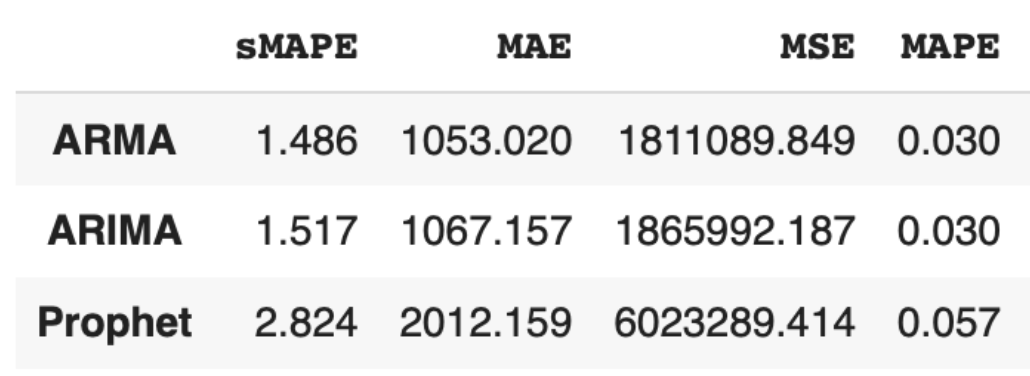
\includegraphics[width=0.8\textwidth]{images/metrcis.png}
\caption{Quality metrics}
\label{fig:figure2}
\end{center}

\end{figure}
\\
It can be concluded that ARMA model, that has the lowest indications for the most of error metrics, is the best model to choose for further predictions.
